\documentclass[aspectratio=169,13pt,fleqn,t] {beamer}
%
% Choose how your presentation looks.
%
% For more themes, color themes and font themes, see:
% http://deic.uab.es/~iblanes/beamer_gallery/index_by_theme.html
%
\mode<presentation>
{
	\usetheme{Madrid}      % 整体主题
	\usecolortheme{beaver} % 配色主题（棕红系）
	\usefonttheme{serif}   % 全局衬线字体（正文宋体类）
	\setbeamertemplate{items}[default] % 【items父模板】控制 itemize+enumerate 符号
%	\setbeamertemplate{items}{\Large\beamertemplateballitem}
	\setbeamertemplate{sections/subsections in toc}[ball] % 目录里章节用圆圈标记
	
	%  \setbeamertemplate{navigation symbols}{} % 取消注释可隐藏底部导航小图标
	\setbeamertemplate{caption}[numbered] % 图/表标题带编号：图1、表1
}

\usepackage[,UTF8,linespread=1.2]{ctex}
\usepackage{wrapfig}
\usepackage{caption}
\usepackage{tcolorbox}
\tcbuselibrary{skins}
\captionsetup[figure]{name=图,labelsep=period}
\usepackage{pdfpages}
\usepackage{tabularx,array}
\usetikzlibrary{arrows.meta,intersections,positioning}
\captionsetup[figure]{,aboveskip=-5pt}

\usepackage{xcolor}
\definecolor{xy_blue}{cmyk}{0.6,0.35,0.0,0.4}
\definecolor{xy_orange}{cmyk}{0.0,0.7,1.0,0.0}
\definecolor{xy_green}{cmyk}{0.2,0.0,1.0,0.15}
\xdefinecolor{xy_gold}{RGB}{135,103,79}
\xdefinecolor{xy2_gold}{cmyk}{0,0.35,0.75,0.05}

\setbeamercolor{section number projected}{fg=red,bg=red!20}%控制球的颜色
\setbeamercolor{subsection number projected}{fg=blue,bg=blue!40}
\setbeamercolor{item}{fg=xy_gold} %设置列表项颜色

\usepackage{amsthm}
\newtheorem{peroration}{结论：}
\newtheorem*{exploration}{探究：}
\newtheorem*{prooft}{证明：}
\newtheorem*{solve}{解:} 
\newtheorem{instance}{例}   % 解：独立计数器
\newtheorem*{definate}{定义：}
\newtheorem{practice}{练习}
\newtheorem{exercise}{习题}
     

% 配色（你前面需要的，每个环境单独颜色）
\setbeamercolor{theorem}{fg=black,bg=blue!10}
\setbeamercolor{solution}{fg=black,bg=green!10}

\BeforeBeginEnvironment{peroration}{%结论： 
	\setbeamercolor{block title}{bg=xy_green,fg=white}
	\setbeamercolor{block body}{bg=xy_green!10}
}
\AfterEndEnvironment{peroration}{
	\setbeamercolor{block title}{bg=xy_blue,fg=white}
	\setbeamercolor{block body}{bg=xy_blue!10}
}
\BeforeBeginEnvironment{exploration}{%探究
	\setbeamercolor{block title}{bg=xy_orange,fg=white}
	\setbeamercolor{block body}{bg=xy_orange!10}
}
\AfterEndEnvironment{peroration}{
	\setbeamercolor{block title}{bg=xy_blue,fg=white}
	\setbeamercolor{block body}{bg=xy_blue!10}
}
\BeforeBeginEnvironment{solution}{%解
	\begingroup
	\setbeamercolor{block title}{bg=xy_green,fg=white}
	\setbeamercolor{block body}{bg=xy_green!10}
}
\AfterEndEnvironment{solution}{
	\endgroup
}
\BeforeBeginEnvironment{prooft}{%证明
	\setbeamercolor{block title}{bg=xy_green,fg=white}
	\setbeamercolor{block body}{bg=xy_green!10}
}
\AfterEndEnvironment{prooft}{
	\setbeamercolor{block title}{bg=xy_green,fg=white}
	\setbeamercolor{block body}{bg=xy_green!10}
}
\BeforeBeginEnvironment{solve}{%解：
	\setbeamercolor{block title}{bg=xy_orange!60,fg=white}
	\setbeamercolor{block body}{bg=xy_orange!10}
}
\AfterEndEnvironment{solve}{%解：
	\setbeamercolor{block title}{bg=xy_orange!60,fg=white}
	\setbeamercolor{block body}{bg=xy_orange!10}
}
   
\BeforeBeginEnvironment{instance}{% 例子
	\begingroup
   	\setbeamercolor{block title}{bg=xy_gold!40,fg=white}
   	\setbeamercolor{block body}{bg=xy_gold!10}
   }
\AfterEndEnvironment{instance}{
	\endgroup
   }     
\BeforeBeginEnvironment{practice}{% 练习
	\begingroup
	\setbeamercolor{block title}{bg=xy_gold!40,fg=white}
	\setbeamercolor{block body}{bg=xy_gold!10}
}
\AfterEndEnvironment{practice}{
	\endgroup
}    

\BeforeBeginEnvironment{exercise}{% 习题
	\begingroup
	\setbeamercolor{block title}{bg=xy_gold!40,fg=white}
	\setbeamercolor{block body}{bg=xy_gold!10}
}
\AfterEndEnvironment{exercise}{
	\endgroup
} 
   
\renewcommand{\thefigure}{\arabic{figure}}

\title[练习及习题答案解析]{P54练习及习题答案解析}
\author[好好学习，努力向上]{}
\institute{}
\date{2026.9.29}
\setbeamertemplate{theorems}[numbered]

\AtBeginSection[]
{
  \begin{frame}<beamer>
    \frametitle{本节主要内容}
    \tableofcontents[currentsection,currentsubsection]
  \end{frame}
}

\AtBeginDocument{
	\setlength{\abovedisplayskip}{3pt}
	\setlength{\belowdisplayskip}{3pt}
	}


\begin{document}
\begin{frame}{}
	\titlepage
\end{frame}

%\begin{frame}{内容概览}
%	\tableofcontents
%\end{frame}

\begin{frame}
	\begin{practice}
		$x$ 是什么实数时，$\sqrt{x^2+x-12}$ 有意义？
	\end{practice}
	
	\begin{solve}
		令 $x^2+x-12\geq 0$，
		
		解得 $x\leq -4$ 或 $x\geq 3$，
		
		即当 $x\leq -4$ 或 $x\geq 3$ 时，$\sqrt{x^2+x-12}$ 有意义。
	\end{solve}
\end{frame}

\begin{frame}
	\begin{practice}
		如图\ref{fig:fig2-3-1}，在长为 $8$ m，宽为 $6$ m 的矩形地面的四周种植花卉，中间种植草坪。如果要求花卉带的宽度相同，且草坪的面积不超过总面积的一半，那么花卉带的宽度应为多少米？
	\end{practice}
	\vspace{-1em}
	\begin{solve}
		\begin{wrapfigure}{r}{5cm}
			\begin{center}			
			
\includegraphics{Figures/budengshi2-3-1.pdf}
			\end{center}
			\caption{}
			\label{fig:fig2-3-1}
		\end{wrapfigure}
		设花带的宽度为 $x$ m，		
		则草坪面积为 $(8-2x)(6-2x)$。
		
		由题意得 $(8-2x)(6-2x)\leq 24$，即 $x^2-7x+6\leq 0$，解得 $1\leq x\leq 6$。		
		又
		\[
		\begin{cases}
			x>0,\\
			8-2x>0,\\
			6-2x>0,
		\end{cases}
		\]
		所以 $0<x<3$，故 $1\leq x<3$。
		
		所以花带的宽度应在 $1$ m 到 $3$ m 之间（包括 $1$ m，不包括 $3$ m）。
	\end{solve}
\end{frame}

\begin{frame}
	\begin{practice}
		某网店销售一批新款削笔器，每个削笔器的最低售价为 $15$ 元。若按最低售价销售，每天能卖出 $30$ 个；若一个削笔器的售价每提高 $1$ 元，日销售量将减少 $2$ 个。为了使这批削笔器每天获得 $400$ 元以上的销售收入，应怎样制定这批削笔器的销售价格？
		
	\end{practice}
	
	\begin{solve}
		
		设每个削笔器的售价为 $x$ 元，由题意得
		\[
		\begin{cases}
			x\geq 15,\\
			x\bigl[30-2(x-15)\bigr]>400,
		\end{cases}
		\]
		解得 $15\leq x<20$。
		
		所以售价应大于或等于 $15$ 元，且小于 $20$ 元。
	\end{solve}
\end{frame}

\begin{frame}
	\begin{exercise}
		求下列不等式的解集：
		\begin{enumerate}[(1)]
			\item $13-4x^2>0$；
			\item  $(x-3)(x-7)<0$；
			\item $x^2-3x-10>0$；
			\item  $-3x^2+5x-4>0$。
		\end{enumerate}
		
		
	\end{exercise}
	
	\begin{solve}
		\begin{enumerate}[(1)]
		
	\item $\left\{x\;\middle|\;-\dfrac{\sqrt{13}}{2}<x<\dfrac{\sqrt{13}}{2}\right\}$。
	
	\item  $\{x\mid 3<x<7\}$。
	
	\item  $\{x\mid x<-2\ \text{或}\ x>5\}$。
	
	\item  $\varnothing$。
	\end{enumerate}
	\end{solve}
\end{frame}

\begin{frame}
	\begin{exercise}
	 $x$ 是什么实数时，下列各式有意义？
	\begin{enumerate}[(1)]
		\item $\sqrt{x^2-4x+9}$；
		\item $\sqrt{-2x^2+12x-18}$。
	\end{enumerate}

	\end{exercise}
	
	\begin{solve}
		\begin{enumerate}[(1)]
			\item 令 $x^2-4x+9=0$，
			
			因为 $\Delta=-20<0$，所以方程 $x^2-4x+9=0$ 无实数根，
			
			所以不等式 $x^2-4x+9\geq 0$ 的解集是 $\mathbf{R}$。
			
			所以当 $x\in\mathbf{R}$ 时，$\sqrt{x^2-4x+9}$ 有意义。
			\item 由题意得 $-2x^2+12x-18\geq 0$，即 $(x-3)^2\leq 0$，
			
			所以当 $x=3$ 时，$\sqrt{-2x^2+12x-18}$ 有意义。
		\end{enumerate}
		
	\end{solve}
\end{frame}

\begin{frame}
	\begin{exercise}
		已知 $M=\{x\mid 4x^2-4x-15>0\}$，$N=\{x\mid x^2-5x-6>0\}$，求 $M\cap N$，$M\cup N$。
	\end{exercise}
	
	\begin{solve}
		由题意得
	\[
	M=\left\{x\;\middle|\;x<-\frac{3}{2}\ \text{或}\ x>\frac{5}{2}\right\},\quad
	N=\{x\mid x<-1\ \text{或}\ x>6\},
	\]
	所以
	\[
	M\cap N=\left\{x\;\middle|\;x<-\frac{3}{2}\ \text{或}\ x>6\right\},
	\]
	\[
	M\cup N=\left\{x\;\middle|\;x<-1\ \text{或}\ x>\frac{5}{2}\right\}.
	\]
	\end{solve}
\end{frame}

\begin{frame}
	\begin{exercise}
	一名同学以初速度 $v_0=12$ m/s 竖直上抛一排球，排球能够在抛出点 $2$ m 以上的位置最多停留多长时间（精确到 $0.01$ s）？
	\end{exercise}
	
	\begin{solve}
		$h=v_0 t-\dfrac{1}{2}\times 10t^2=12t-5t^2$，
		
		由 $h>2$ 得 $12t-5t^2>2$，即 $5t^2-12t+2<0$，解得
		\vspace{3pt}
		\[
		\frac{6-\sqrt{26}}{5}<t<\frac{6+\sqrt{26}}{5},
		\]
		\addvspace{5pt}
		即 $\dfrac{6+\sqrt{26}}{5}-\dfrac{6-\sqrt{26}}{5}=2.04$（s），
		
		最多停留 $2.04$ s。
	\end{solve}
\end{frame}

\begin{frame}
	\begin{exercise}
		已知集合 $A=\{x\mid x^2-16<0\}$，$B=\{x\mid x^2-4x+3>0\}$，求 $A\cup B$。
	\end{exercise}
	
	\begin{solve}
		因为 $A=\{x\mid x^2-16<0\}=\{x\mid -4<x<4\}$，$B=\{x\mid x^2-4x+3\geq 0\}=\{x\mid x\leq 1\ \text{或}\ x\geq 3\}$，
		
		所以 $A\cup B=\{x\mid -4<x<4\}\cup\{x\mid x\leq 1\ \text{或}\ x\geq 3\}=\mathbf{R}$。
	\end{solve}
\end{frame}

\begin{frame}
	\vspace{-1em}
	\begin{exercise}

	如图\ref{fig:fig2-3-2}，据气象部门预报，在距离某码头南偏东 $45^\circ$ 方向 $600$ km 处的热带风暴中心正以 $20$ km/h 的速度向正北方向移动，距风暴中心 $450$ km 以内的地区都将受到影响。据以上预报估计，从现在起多长时间后，该码头将受到热带风暴的影响，影响时间大约为多长（精确到 $0.1$ h）？
	\end{exercise}
\vspace{-1em}
	\begin{minipage}{0.65\textwidth}
		\begin{solve}			
			设风暴中心坐标为 $(a,b)$，则 $a=300\sqrt{2}$，所以 $\sqrt{(300\sqrt{2})^2+b^2}<450$，即 $-150<b<150$。而
			\[
			\frac{300\sqrt{2}-150}{20}=\frac{15}{2}(2\sqrt{2}-1)\approx 13.7,
			\]
			\[
			\frac{300}{20}=15,
			\]
			所以大约经过 $13.7$ 小时后码头将受到热带风暴的影响，影响时间为 $15.0$ 小时。
		\end{solve}
	\end{minipage}%	
	\begin{minipage}{0.4\textwidth}
	\begin{figure}[h]
		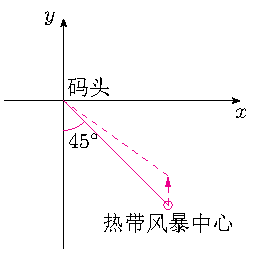
\includegraphics{Figures/budengshi2-3-2.pdf}
		\caption{}
		\label{fig:fig2-3-2}
		\end{figure}
	\end{minipage}

\end{frame}
\end{document}
